\documentclass[a4paper,12pt]{article}
\usepackage{../packages/coursCollege}
\newcommand{\Chapitre}{Limites}
\renewcommand{\path}{../../}

\renewcommand{\cours}{3MA1~--~EG~--~ns~--~2025-2026}
\begin{document}

\section{Activités}
\section{Définition non formelle -- notion intuitive}
\begin{definition}
	\tcblower
	Un \emph{voisinage} d'un nombre réel $a$ est un intervalle ouvert qui contient $a$.
\end{definition}
\begin{exemple}
	Voisinages de $3$
	\tcblower
		Les intervalles ouverts $]1\,{;}\,4[$ et $]2{,}9999\,{;}\,3{,}000000001[$ sont des voisinages de $3$.
\end{exemple}
\begin{remarque}
	\tcblower
 Par définition, un voisinage d'un nombre réel $a$ contient une infinité de nombres plus petit et plus grand que $a$. 
\end{remarque}
\begin{definition}
	\tcblower
	On dit qu'une fonction est \emph{définie au voisinage} d'un nombre réel $a$, s'il existe un voisinage de $a$ sur lequel la fonction est définie, sauf peut-être en~$a$.
\end{definition}

\begin{definition}
$x\rightarrow~a^-$
	\tcblower
	Soit $a$ nombre réel.
	Lorsqu'on écrit \emph{«~$x$ tend vers $a$ par la gauche~»} cela signifie que $x$ s'approche autant qu'on veut de $a$ par des valeurs inférieures à $a$, tout en restant toujours différent de $a$. 

On note $x\rightarrow~a^-$.
\end{definition}

\begin{definition}
$x\rightarrow a^+$
	\tcblower
	Soit $a$ nombre réel.
	Lorsqu'on écrit \emph{«~$x$ tend vers $a$ par la droite~»} cela signifie que $x$ s'approche autant qu'on veut de $a$ par des valeurs supérieures à $a$, tout en restant toujours différent de $a$. 

	On note $x\rightarrow a^+$.
\end{definition}
\begin{definition}
 $x\rightarrow a$
	\tcblower
	Soit $a$ nombre réel.
	Lorsqu'on écrit \emph{«~$x$ tend vers $a$~»} cela signifie que $x$ s'approche autant qu'on veut de $a$ par des valeurs inférieures ou supérieures à $a$, tout en restant toujours différent de $a$.

\noindent	On note $x\rightarrow a$.
\end{definition}
\begin{definition}
$\displaystyle{\lim_{x\rightarrow a^-}f(x)=\ell}$

$\displaystyle{\lim_{\substack{x\to a \\ x<a}}f(x)=\ell}$
	\tcblower
Soit $f$ une fonction définie au voisinage d'un nombre $a$ et soit $\ell$ un nombre réel ou le symbole $-\infty$, $+\infty$. On dit que \emph{«~la limite à gauche de $f(x)$ quand $x$ tend vers $a$ vaut $\ell$~»} si $f(x)$ s'approche «~aussi près qu'on veut~» de $\ell$ lorsque $x\rightarrow a^-$.

On écrit $\displaystyle{\lim_{x\rightarrow a^-}f(x)=\ell}$ ou encore $\displaystyle{\lim_{\substack{x\to a \\ x<a}}f(x)=\ell}$. 
\end{definition}
\begin{definition}
$\displaystyle{\lim_{x\rightarrow a^+}f(x)=\ell}$

$\displaystyle{\lim_{\substack{x\to a \\ x>a}}f(x)=\ell}$
	\tcblower
Soit $f$ une fonction définie au voisinage d'un nombre $a$ et soit $\ell$ un nombre réel ou le symbole $-\infty$, $+\infty$. On dit que \emph{«~la limite à droite de $f(x)$ quand $x$ tend vers $a$ vaut $\ell$~»} si $f(x)$ s'approche «~aussi près qu'on veut~» de $\ell$ lorsque $x\rightarrow a^+$.

On écrit $\displaystyle{\lim_{x\rightarrow a^+}f(x)=\ell}$ ou encore $\displaystyle{\lim_{\substack{x\to a \\ x>a}}f(x)=\ell}$. 
\end{definition}
\begin{exemple}[label=ex:fmorceaux]
Soit la fonction $f$ définie par 
\[f(x)=\begin{cases}x^2+1 & \text{si } x>1\\
5-x& \text{si } x\leq 1
\end{cases}. \]
Déterminer graphiquement $\displaystyle{\lim_{x\rightarrow 1^{-}}} f(x)$ et $\displaystyle{\lim_{x\rightarrow 1^{+}}f(x)}$.
\tcblower  
On commence par représenter graphiquement $f$. 

\begin{center}
		\begin{tikzpicture}[scale=1]
  \begin{axis}[
    axis lines=middle,
    xlabel={$x$}, ylabel={$y$},
    xlabel style={at=(current axis.right of origin), anchor=west},
    ylabel style={at=(current axis.above origin), anchor=south},
    xmin=-2, xmax=2.5, ymin=0, ymax=5,
    xtick={-2,-1,0,1,2},
    ytick={0,1,2,3,4,5},
    samples=200,
  ]
    % curved branch: x^2+1 for x<=1
    \addplot [domain=-2:1, thick] {x*x+1} node[below left,pos=0.5] {$f(x)$};
    % straight branch: 5-x for x>1
    \addplot [domain=1:5, thick] {5-x};
    % filled dot at (1,2)
    \addplot[only marks, mark=*, mark size=2pt] coordinates {(1,2)};
    % open dot at (1,4)
    \addplot[only marks, mark=o, mark size=2pt] coordinates {(1,4)};
    % dashed guide‐lines
    \draw[dashed] (axis cs:1,0) -- (axis cs:1,2);
    \draw[dashed] (axis cs:0,2) -- (axis cs:1,2);
    \draw[dashed] (axis cs:1,0) -- (axis cs:1,4);
    \draw[dashed] (axis cs:0,4) -- (axis cs:1,4);
  \end{axis}
\end{tikzpicture}
\end{center}
On observe que $\displaystyle{\lim_{x\rightarrow 1^{-}}f(x)}=2$ et que $\displaystyle{\lim_{x\rightarrow 1^{+}}f(x)}=4$.  

Pour rappel, ce type de fonction est une fonction définie par morceaux. 
\end{exemple}

\begin{definition}
$\displaystyle{\lim_{x\rightarrow a}f(x)=\ell}$
	\tcblower
	Soient une fonction $f$, un nombre $a$ et $\ell$ un nombre ou le symbole $-\infty$, $+\infty$. 
On dit que \emph{«~la limite de $f(x)$ quand $x$ tend vers $a$ existe et vaut $\ell$~»} si $f(x)$ s'approche «~aussi près qu'on veut~» de $\ell$ lorsque $x\rightarrow a$.

On écrit $\displaystyle{\lim_{x\rightarrow a}f(x)=\ell}$. \end{definition}

\begin{thm}[label=thm:unicite]
	Unicité de la limite
	\tcblower
Si $\displaystyle{\lim_{x\rightarrow a}f(x)=\ell}$ existe, alors elle est unique.	
\end{thm}

\begin{thm}
	Existence de la limite
\tcblower
Une limite existe si et seulement si les limites à gauche et à droite sont égales, i.e.

\[\displaystyle{\lim_{x\rightarrow a}f(x)=\ell} \iff \displaystyle{\lim_{x\rightarrow a^-}f(x)}= \displaystyle{\lim_{x\rightarrow a^+}f(x)=\ell}.\]
\end{thm}
\begin{exemple}
	\tcblower
	Dans l'exemple \ref{ex:fmorceaux}, la fonction $f$ n'admet pas de limite en $1$, car par la contraposée du théorème \ref{thm:unicite} la limite à gauche et la limite à droite ne sont pas égales.  
\end{exemple}
\begin{exemple}
	Soit $f$ définie par \[f(x)=\begin{cases}x+1& \text{si } x<3\\ -2x+7 & \text{si } x\geq 3\end{cases}\]	
	Déterminer $\displaystyle{\lim_{x\rightarrow 3}f(x)}$. 
	\tcblower
	On représente graphiquement $f$.
\begin{center}
\begin{tikzpicture}
  \begin{axis}[
    axis lines=middle,
    xlabel={$x$}, ylabel={$y$},
    xlabel style={at=(current axis.right of origin), anchor=west},
    ylabel style={at=(current axis.above origin), anchor=south},
    xmin=-2, xmax=7, ymin=-2, ymax=5,
    xtick={-2,0,2,4,6},
    ytick={-2,0,2,4},
    grid=both,
    grid style={dashed,gray!30},
  ]
    \addplot [domain=-2:3, thick] {x+1}
      node[above left,pos=0.8] {$f(x)$};
    \addplot [domain=3:7, thick] {-2*x+7};
    % open and closed points at x=3
    \addplot [only marks, mark=o, thick] coordinates {(3,4)};
    \addplot [only marks, mark=*, thick] coordinates {(3,1)};
  \end{axis}
\end{tikzpicture}\end{center}
 On observe que 
	\[\lim_{x\rightarrow 3^+}f(x)=4 \quad \text{et} \quad \lim_{x\rightarrow 3^-}f(x)=1\]
	donc la limite $\displaystyle{\lim_{x\rightarrow 3}f(x)}$ n'existe pas.
\end{exemple}
\begin{exemple}
	Soit la fonction $f$ définie par $f(x)=\dfrac{9-x}{3-\sqrt{x}}$. Étudier graphiquement $\displaystyle{\lim_{x\rightarrow 9}f(x)}$ et $\displaystyle{\lim_{x\rightarrow 4}f(x)}$. 
	\tcblower
	On remarque que le domaine de définition de $f$ est 
$D_f=\mathbb{R}\setminus\{9\}$. On représente la fonction graphiquement. 
\begin{center}
	\begin{tikzpicture}
  \begin{axis}[
    axis lines=middle,
    xlabel={$x$}, ylabel={$y$},
    xlabel style={at=(current axis.right of origin), anchor=west},
    ylabel style={at=(current axis.above origin), anchor=south},
    xmin=0,   xmax=15,
    ymin=0,   ymax=9,
    xtick={0,4,9,15},
    ytick={0,5,6,8},
    grid=both,
    grid style={dashed,gray!30},
  ]
    % branche pour 0 ≤ x < 9
    \addplot[domain=0:8.9, samples=200, thick]
      {(9 - x)/(3 - sqrt(x))};
    % branche pour x > 9
    \addplot[domain=9.1:15, samples=200, thick]
      {(9 - x)/(3 - sqrt(x))}
      node[above,pos=0.5] {$f(x)$};
    % point ouvert en (9,6)
    \addplot[only marks, mark=o, thick] coordinates {(9,6)};
    % point fermé en (4,5)
    \addplot[only marks, mark=*, thick] coordinates {(4,5)};
    % traits pointillés illustrant les limites/valeurs
    \draw[dashed] (axis cs:0,6) -- (axis cs:9,6);
    \draw[dashed] (axis cs:9,0) -- (axis cs:9,6);
    \draw[dashed] (axis cs:0,5) -- (axis cs:4,5);
    \draw[dashed] (axis cs:4,0) -- (axis cs:4,5);
  \end{axis}
\end{tikzpicture}
\end{center}
On a $\displaystyle{\lim_{x\rightarrow 9}f(x)=6}$ même si $f$ n'est pas définie en $9$ (indiqué par le rond vide). De plus $\displaystyle{\lim_{x\rightarrow 4}f(x)=5}$. On a calculé les deux limites et on a montré qu'elles existent.  
\end{exemple}
\begin{exemple}
	Soit $f$ définie par $f(x)=\dfrac{x^3-1}{x^2-1}$. Déterminer $\displaystyle{\lim_{x\rightarrow 1}f(x)}$ et $\displaystyle{\lim_{x\rightarrow -1}f(x)}$.
	\tcblower
	On commence par remarquer que $D_f=\mathbb{R}\setminus\{-1\}$. On représente graphiquement $f$. 
	\begin{center}
		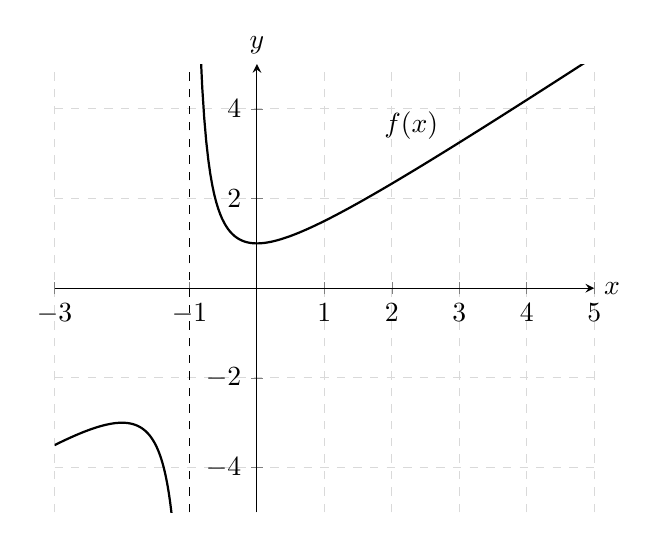
\begin{tikzpicture}
  \begin{axis}[
    axis lines=middle,
    xlabel={$x$}, ylabel={$y$},
    xlabel style={at=(current axis.right of origin), anchor=west},
    ylabel style={at=(current axis.above origin), anchor=south},
    xmin=-3, xmax=5, ymin=-5, ymax=5,
    xtick={-3,-1,0,1,2,3,4,5},
    ytick={-4,-2,0,2,4},
    grid=both,
    grid style={dashed,gray!30},
  ]
    % branche pour x < -1
    \addplot [domain=-3:-1.1, samples=200, thick]
      {(x^3-1)/(x^2-1)};
    \addplot [domain=-0.9:5, samples=200, thick]
      {(x^3-1)/(x^2-1)} node[above left,pos=0.8] {$f(x)$};
    % asymptote verticale en x = -1
    \draw[dashed] (axis cs:-1,-5) -- (axis cs:-1,5);
  \end{axis}
\end{tikzpicture}
	\end{center}
	On observe que 
	\[\displaystyle{\lim_{x\rightarrow 1^-}f(x)=\dfrac{3}{2}} \quad \text{et} \quad \displaystyle{\lim_{x\rightarrow 1^+}f(x)=\dfrac{3}{2}}\]
	donc $\displaystyle{\lim_{x\rightarrow 1}f(x)}$ existe et vaut $\dfrac{3}{2}$. Toutefois, 
	\[\displaystyle{\lim_{x\rightarrow -1^-}f(x)=-\infty} \quad \text{et} \quad \displaystyle{\lim_{x\rightarrow -1^+}f(x)=+\infty}\]
	donc $\displaystyle{\lim_{x\rightarrow -1}f(x)}$ n'existe pas.
\end{exemple} 
\begin{autre}
	\tcblower

\end{autre}
Il existe une définition plus formelle des limites, mais elle sort du cadre de ce cours. Nous verrons à présent des outils pour calculer plus formellement des limites. Certains des résultats seront démontrés et d'autres seront acceptés sans démonstration.
\section{Limites de fonctions élémentaires}
\begin{thm}[label=thm:limel]
Limites de fonctions élémentaires

(sans démonstration)
	\tcblower
	\noindent\begin{description}
		\item[{\bfseries L1}] Si $k\in\mathbb{R}$, alors $\displaystyle{\lim_{x\rightarrow a}k=k}, \,\forall a\in\mathbb{R}$
		\item[{\bfseries L2}] Si $x\in \mathbb{R}$, alors $\displaystyle{\lim_{x\rightarrow a}x=a}, \,\forall a\in \mathbb{R}$
		\item[{\bfseries L3}] Si $x\in \mathbb{R}$, alors $\displaystyle{\lim_{x\rightarrow a}\sin(x)=\sin(a)}$ et $\displaystyle{\lim_{x\rightarrow a}\cos(x)=\cos(a)},\, \forall a\in \mathbb{R}$
		\item[{\bfseries L4}] Si $f(x)=\sqrt[n]{x}$ et $D_f$ est son domaine de définition, 

			alors $\displaystyle{\lim_{x\rightarrow a}\sqrt[n]{x}=\sqrt[n]{a}}, \, \forall a \in D_f$ 
		\item[{\bfseries L5}] Si $b\in \mathbb{R}_{>0}\setminus\{1\}$, alors $\displaystyle{\lim_{x\rightarrow a}\log_b(x)=\log_b(a)}, \,\forall a\in \mathbb{R}_{>0}$ et 

			$\displaystyle{\lim_{x\rightarrow a}\exp_b(x)=\exp_b(a)},\,\forall a\in \mathbb{R}$  	
	\end{description}
\end{thm}
\begin{exemple}
	Calculer $\displaystyle{\lim_{x\rightarrow -3}14}$
	\tcblower
	$\displaystyle{\lim_{x\rightarrow -3}14\stackrel{\text{{\bfseries L1}}}{=}14}$, par la première limite du théorème \ref{thm:limel}. 
\end{exemple}

\begin{exemple}
	Calculer $\displaystyle{\lim_{x\rightarrow 5}x}$
	\tcblower
	$\displaystyle{\lim_{x\rightarrow 5}x\stackrel{\text{{\bfseries L2}}}{=}5}$ 
\end{exemple}

\begin{exemple}
	Calculer $\displaystyle{\lim_{x\rightarrow \frac{\pi}{2}}\sin(x)}$
	\tcblower
	$\displaystyle{\lim_{x\rightarrow \frac{\pi}{2}}\sin(x)\stackrel{\text{{\bfseries L3}}}{=}\sin\left(\frac{\pi}{2}\right)}=1$ 
\end{exemple}
\begin{exemple}
	Calculer $\displaystyle{\lim_{x\rightarrow 8}\sqrt[3]{x}}$
	\tcblower
	$\displaystyle{\lim_{x\rightarrow 8}\sqrt[3]{8}\stackrel{\text{{\bfseries L4}}}{=}\sqrt[3]{8}=2}$ 
\end{exemple}
\begin{exemple}
	Calculer $\displaystyle{\lim_{x\rightarrow 32}\log_2(x)}$
	\tcblower
	$\displaystyle{\lim_{x\rightarrow 32}\log_2(x)\stackrel{\text{{\bfseries L5}}}{=}\log_2(32)=\log_2\left(2^5\right)=5}$ 
\end{exemple}

\section{Propriétés des limites}
Les propriétés suivantes nous permettent de calculer des limites plus compliquées du type $\displaystyle{\lim_{x\rightarrow 2}\dfrac{x-5}{x}}$.
\begin{remarque}
	\tcblower
	Pour rappel, une limite existe, si \[ \displaystyle{\lim_{x\rightarrow a^-}f(x)}= \displaystyle{\lim_{x\rightarrow a^+}f(x)=\ell}\]
	pour $\ell$ un nombre ou le symbole $-\infty$, $+\infty$.
\end{remarque}
\begin{thm}
	Propriétés des limites

	(sans démonstration)
	\tcblower
Si $\displaystyle{\lim_{x\rightarrow a}f(x)}$ et $\displaystyle{\lim_{x\rightarrow a}g(x)}$ existent, alors on a 
\noindent
\begin{description}
	\item[{\bfseries P0}] $\displaystyle{\lim_{x\rightarrow a}k\cdot f(x)=k\cdot \lim_{x\rightarrow a}f(x)},\, \forall k\in \mathbb{R}$ 
	\item[{\bfseries P1}] $\displaystyle{\lim_{x\rightarrow a}\left(f(x)+g(x)\right)=\lim_{x\rightarrow a}f(x)+\lim_{x\rightarrow a}g(x)}$ 
	\item[{\bfseries P2}] $\displaystyle{\lim_{x\rightarrow a}\left(f(x)-g(x)\right)=\lim_{x\rightarrow a}f(x)-\lim_{x\rightarrow a}g(x)}$ 
	\item[{\bfseries P3}] $\displaystyle{\lim_{x\rightarrow a}\left(f(x)\cdot g(x)\right)=\lim_{x\rightarrow a}f(x)\cdot \lim_{x\rightarrow a}g(x)}$ 
	\item[{\bfseries P4}] $\displaystyle{\lim_{x\rightarrow a}\dfrac{f(x)}{g(x)}=\dfrac{\lim_{x\rightarrow a}f(x)}{\lim_{x\rightarrow a}g(x)}}$ 
\end{description}
\end{thm}
\begin{thm}[label=thm:compo]
	Limite d'une composition
	\tcblower
	Si $\displaystyle{\lim_{x\rightarrow a}f(x)=b}$ et $\displaystyle{\lim_{t\rightarrow b}g(t)=g(b)}$ existent, alors on a~:
	\[\lim_{x\rightarrow a}g(f(x))=g(\lim_{x\rightarrow a }f(x))=g(b).\] 
\end{thm}
\begin{thm}[label=thm:poly]
Limites de fonctions polynômiales	
	\tcblower
	Si $f$ est une fonction polynomiale, i.e. 
	\[f(x)=a_nx^n+a_{n-1}x^{n-1}+\ldots+a_2 x^2+a_1x_1+a_0,\]
	alors, pour $b\in\mathbb{R}$, on a~:
	\[\lim_{x\rightarrow b}f(x)=f(b)=a_n b^n+\ldots+a_1b+a_0.\]
\begin{proof}
On a $\displaystyle{\lim_{x\rightarrow b}x}\stackrel{\text{{\bfseries L2}}}{=}b$. De plus, pour tout $m\in \mathbb{N}$, 

\[\displaystyle{\lim_{x\rightarrow b}x^m\stackrel{\text{\bfseries P3}}{=}}\left(\displaystyle{\lim_{x\rightarrow b}x}\right)^m=b^m.\] 

Ainsi,

\begin{align*}
	\lim_{x\rightarrow b} \left(a_nx^n+\ldots +a_1x_1+a_0\right)&\stackrel{\text{{\bfseries P2}}}{=}\lim_{x\rightarrow b} a_nx^n+\ldots+\lim_{x\rightarrow b} a_1x+\lim_{x\rightarrow b}a_0\\
									     &\stackrel{\text{{\bfseries P0 et L2}}}{=}a_n\lim_{x\rightarrow b} x^n+\ldots+a_1\cdot\lim_{x\rightarrow b} x+a_0\\							     
									     &\stackrel{\text{{\bfseries P3}}}{=}a_n b^n+\ldots+a_1b+a_0.
\end{align*}


\end{proof}
\end{thm}

\begin{thm}
	\tcblower
	Soient $f$ et $g$ deux fonctions définies sur un voisinage $I$ de $a\in \mathbb{R}$ telles que  
	\begin{tasks}
		\task $f(x)\leq g(x),\, \forall x \in I$
		\task $\displaystyle{\lim_{x\rightarrow a}f(x)}$ et $\displaystyle{\lim_{x\rightarrow a}g(x)}$ existent  
	\end{tasks} alors 

	\[\displaystyle{\lim_{x\rightarrow a}f(x)}\leq  \displaystyle{\lim_{x\rightarrow a}g(x)}, \forall a\in I\]

	($a$ peut également valoir $-\infty$ et $\infty$ si l'intervalle $I$ n'est pas borné).
\end{thm}
\begin{thm}
	Théorème des gendarmes
	\tcblower
	Soient $f, g$ et $h$ des fonctions définies sur un voisinage $I$ de $a\in \mathbb{R}$ ($a$ peut également valoir $-\infty$ ou $\infty$) telles que
	\begin{tasks}
		\task $f(x)\leq g(x)\leq h(x),\, \forall x \in I$
		\task $\displaystyle{\lim_{x\rightarrow a}f(x)}=\displaystyle{\lim_{x\rightarrow a}h(x)}=\ell$ 

		($\ell$ peut également être égal au symbole $-\infty$ ou $\infty$).  
	\end{tasks} alors 

	\[\displaystyle{\lim_{x\rightarrow a}g(x)}=\ell.\]
\end{thm}
\begin{exemple}
$\displaystyle{\lim_{x\to2}\left(\frac{x-5}{x}\right)}$
	\tcblower
On peut maintenant calculer la limite considérée en introduction en justifiant le calcul :
	\[\lim_{x\to2}\left(\frac{x-5}{x}\right)
		\stackrel{\text{{\bfseries P4}}}{=}
\dfrac{\displaystyle{\lim_{x\to2}(x-5)}}{\displaystyle{\lim_{x\to2}x}}
\stackrel{\text{{\bfseries {P2}}}}{=}
\dfrac{\displaystyle{\lim_{x\to2}x-\lim_{x\to2}5}}{\displaystyle{\lim_{x\to2}x}}
\stackrel{\text{{\bfseries {L2,L1}}}}{=}
\dfrac{2-5}{2}
=-\dfrac{3}{2}
\]
\end{exemple}


\begin{exemple}
	\begin{tasks}
		\task \(\displaystyle\lim_{x\to-4}(x+3)\)\\
\task \(\displaystyle\lim_{x\to1}2x^2\)\\
\task \(\displaystyle\lim_{x\to2}\frac{x+5}{x}\)\\ 
\task \(\displaystyle\lim_{x\to0}\cos(x^4)\)\\
	\end{tasks}
\tcblower
Calculer en justifiant 
\begin{tasks}
	\task
\[
\lim_{x\to-4}(x+3)
\stackrel{\text{{\bfseries{P1}}}}{=}
\lim_{x\to-4}x+\lim_{x\to-4}3
\stackrel{\text{{\bfseries{L2,L1}}}}{=}
-4+3=-1
\]
ou plus directement :
\[
\lim_{x\to-4}(x+3)
\stackrel{\text{{\bfseries{thm \ref{thm:poly}}}}}{=}
-4+3=-1
\]


\task 

\[
\lim_{x\to1}2x^2
\stackrel{\text{{\bfseries{P0}}}}{=}
2\cdot\lim_{x\to1}x^2
\stackrel{\text{{\bfseries{P3}}}}{=}
2\cdot\lim_{x\to1}x\cdot\lim_{x\to1}x
\stackrel{\text{{\bfseries{L2,L1}}}}{=}
2\cdot1\cdot1=2
\]
ou plus directement :
\[
\lim_{x\to1}2x^2
\stackrel{\text{{\bfseries{thm \ref{thm:poly}}}}}{=}
2\cdot1\cdot1=2
\]
\task 
\[
\lim_{x\to2}\frac{x+5}{x}
\stackrel{\text{{\bfseries{P4}}}}{=}
\frac{\lim_{x\to2}(x+5)}{\lim_{x\to2}x}
\stackrel{\text{{\bfseries thm. \ref{thm:poly},L2}}}{=}
\frac{2+5}{2}
=\frac{7}{2}
\]
\task
\[
\lim_{x\to0}\cos(x^4)
\stackrel{\text{{\bfseries{thm \ref{thm:poly}}}}}{=}
\cos\bigl(\lim_{x\to0}x^4\bigr)
\stackrel{\text{{\bfseries thm \ref{thm:compo}}}}{=}
\cos(0^4)=\cos(0)=1
\]
\end{tasks}
\end{exemple}

\begin{remarque}
	\tcblower
Ces théorèmes montrent que dans de très nombreux cas, la limite de \(f(x)\) quand \(x\) tend vers \(a\) est égale à \(f(a)\), ce qu’on note
\[
\lim_{x\to a}f(x)=f(a);
\]
dans tous ces cas « simples », le comportement de \(f\) près de \(a\) est le même que celui de \(f\) en \(a\). Ce n’est donc pas pour ce type de fonctions que l’« outil limite » est pertinent, mais pour ceux de la section suivante…

Plus tard dans le cours,nous reviendrons sur cette remarque qui nous permettra d’appréhender une notion très importante, {\bfseries la continuité}.
\end{remarque}

\section{Limites infinies -- type $\dfrac{1}{0}$}
\begin{definition}
	Limite infinie
	\tcblower
Soit $f$ une fonction définie au voisinage d’un nombre $a$.

On dit que la limite de $f(x)$ en $a$ est égale à (plus) l’infini si $f(x)$ devient infiniment grand lorsque $x$ se rapproche suffisamment près de $a$ mais sans être égal à $a$.

On écrit :
\[
\lim_{x\to a}f(x)=+\infty
\quad(\text{ou }=\infty)
\]

On dit que la limite de $f(x)$ en $a$ est égale à moins l’infini si $f(x)$ devient infiniment petit lorsque $x$ se rapproche suffisamment près de $a$ mais sans être égal à $a$.

On écrit :
\[
\lim_{x\to a}f(x)=-\infty
\]
\end{definition}
\begin{remarque}
	\tcblower

De la même manière, on peut définir
\[
\lim_{x\to a^+}f(x)=+\infty,\quad
\lim_{x\to a^+}f(x)=-\infty,\quad
\lim_{x\to a^-}f(x)=+\infty,\quad
\lim_{x\to a^-}f(x)=-\infty.
\]
\end{remarque}
\begin{exemple}
Étudier \(\displaystyle\lim_{x\to0}\dfrac1x\) via une approche graphique.
\begin{tikzpicture}[scale=0.6]
  \begin{axis}[
    axis lines=middle,
    xlabel={}, ylabel={},
    xlabel style={at=(current axis.right of origin), anchor=west},
    ylabel style={at=(current axis.above origin), anchor=south},
    xmin=-3, xmax=3, ymin=-4, ymax=4,
    xtick={-3,-2,-1,1,2,3},
    ytick={-4,-2,2,4},
      yticklabel=\empty,
      xticklabel=\empty,
    %grid=both,
    grid style={dashed,gray!30},
  ]
    % branches of 1/x
    \addplot [domain=-3:-0.1,samples=200, thick] {1/x};
    \addplot [domain=0.1:3, samples=200, thick] {1/x}
      node[above right,pos=0.8] {$f(x)=\tfrac1x$};
    % asymptotes
    \draw[dashed] (axis cs:0,-4) -- (axis cs:0,4);
    \draw[dashed] (axis cs:-3,0) -- (axis cs:5,0);
  \end{axis}
\end{tikzpicture}
	\tcblower


Soit \(f\) définie par \(f(x)=\dfrac1x\) :
\[
\lim_{x\to0^-}\dfrac1x
=\dfrac{1}{0^-}=-\infty,\quad
\lim_{x\to0^+}\dfrac1x
=\dfrac{1}{0^+}=+\infty,\]
donc
\[
\lim_{x\to0}\dfrac1x
\text{ n'existe pas.}
\]
\end{exemple}
\begin{exemple}
Étudier\(\displaystyle\lim_{x\to0}\dfrac1{x^2}\) via une approche graphique.
% f(x) = 1/x^2
\begin{tikzpicture}[scale=0.6]
  \begin{axis}[
    axis lines=middle,
    xlabel={}, ylabel={},
    xlabel style={at=(current axis.right of origin), anchor=west},
    ylabel style={at=(current axis.above origin), anchor=south},
    xmin=-3, xmax=3, ymin=-4, ymax=4,
    xtick={-3,-2,-1,1,2,3},
    ytick={-4,-2,2,4},
      yticklabel=\empty,
      xticklabel=\empty,
    %grid=both,
    grid style={dashed,gray!30},
  ]
    % branches of 1/x
    \addplot [domain=-3:-0.1,samples=200, thick] {1/(x*x)};
    \addplot [domain=0.1:3, samples=200, thick] {1/(x*x)}
	    node[above left,pos=1] {$f(x)=\dfrac{1}{x^2}$};
    % asymptotes
    \draw[dashed] (axis cs:0,-4) -- (axis cs:0,4);
    \draw[dashed] (axis cs:-3,0) -- (axis cs:5,0);
  \end{axis}
\end{tikzpicture}	\tcblower

Soit \(f\) définie par \(f(x)=\dfrac1{x^2}\) :
\[
\lim_{x\to0^-}\dfrac1{x^2}
=\dfrac{1}{(0^-)^2}=+\infty,\quad
\lim_{x\to0^+}\dfrac1{x^2}
=\dfrac{1}{(0^+)^2}=+\infty,
\]
donc
\[
\lim_{x\to0}\dfrac1{x^2}=+\infty.
\]
\end{exemple}

\begin{definition}
	Type $«~\dfrac{1}{0}~»$
	\tcblower
	Une limite du type quotient \(\displaystyle \lim_{x\to a}\frac{f(x)}{g(x)}\) pour laquelle on a \(\displaystyle \lim_{x\to a}g(x)=0\) mais où \(\displaystyle \lim_{x\to a}f(x)\neq0\) est appelée limite de type \(«~\displaystyle \frac{1}{0}~»\). 
\end{definition}
\begin{remarque}
	\tcblower
Pour calculer une limite du type \(«~\displaystyle\frac{1}{0}~»\), on doit toujours calculer distinctement la limite à gauche et la limite à droite. Le plus souvent, une factorisation est très utile car nous pouvons ainsi utiliser la règle des signes pour contrôler le signe du résultat. Si les limites à gauche et à droite sont égales, la limite existe et vaut cette valeur ; sinon, elle n'existe pas.
\end{remarque}

\begin{exemple}[label=ex:inf1]
	Calculer  \(\displaystyle\lim_{x\to -2}\frac{-2}{2x+4}\) et interpréter graphiquement.
	\tcblower
\[
\lim_{x\to -2}\frac{-2}{2x+4}
=«~\frac{-2}{0}~»
\,: \text{c'est un type }«~\frac{1}{0}~»;
\]
\[
\lim_{x\to -2^+}\frac{-2}{2x+4}
=\lim_{x\to -2^+}\frac{-2}{2(x+2)}
=\lim_{x\to -2^+}\frac{-1}{x+2}
=«~\frac{-1}{0^+}~»
=-\infty,
\]
et
\[
\lim_{x\to -2^-}\frac{-2}{2x+4}
=«~\frac{-1}{0^-}~»
=+\infty
\]
d'où $\displaystyle{\lim_{x\to -2}\frac{-2}{2x+4}}$ n'existe pas. 
\end{exemple}
\begin{exemple}[label=ex:inf2]
	Calculer  \(\displaystyle\lim_{x\to -2}\frac{-2}{(x+2)^2}\) et interpréter graphiquement.
	\tcblower
\[
\lim_{x\to -2}\frac{-2}{(x+2)^2}
=«~\frac{-2}{0}~»
\,: \text{c'est un type }«~\frac{1}{0}~»
;
\]
\[
\lim_{x\to -2^-}\frac{-2}{(x+2)^2}
=«~\frac{-2}{(0^-)^2~»
}
=-\infty \text{ et } 
\lim_{x\to -2^+}\frac{-2}{(x+2)^2}
=«~\frac{-2}{(0^+)^2~»
}
=-\infty,
\]
\[
\text{donc }\lim_{x\to -2}\frac{-2}{(x+2)^2}=-\infty.
\]
\end{exemple}
\begin{exemple}[label=ex:inf3]
	Calculer \(\displaystyle\lim_{x\to 1}\frac{x-2}{x^2+3x-4}\) et interpréter graphiquement.
	\tcblower
\[
\lim_{x\to 1}\frac{x-2}{x^2+3x-4}
=«~\frac{-1}{0}~»
\,: \text{c'est un type }«~\frac{1}{0}~»
;
\]
\[
\lim_{x\to 1^+}\frac{x-2}{x^2+3x-4}
=\lim_{x\to 1^+}\frac{x-2}{(x-1)(x+4)}
=«~\frac{-1}{0^+\cdot5}~»
=-\infty\]
et
\[
\lim_{x\to 1^-}\frac{x-2}{x^2+3x-4}
=«~\frac{-1}{0^-\cdot5}~»
=+\infty,
\]
\[
	\text{donc }\lim_{x\to 1}\frac{x-2}{x^2+3x-4}\text{ n'existe pas }.
\]
\end{exemple}



Interprétations graphiques :
\begin{center}
	\begin{tikzpicture}[scale=0.7]
    \begin{axis}[
	    axis lines=middle, xlabel={}, ylabel={},
      xmin=-5, xmax=1, ymin=-7, ymax=7,
      samples=200
    ]
    \node[anchor=north west] at (rel axis cs:0,1) {\bfseries Exemple \ref{ex:inf1}};
      \addplot[domain=-5:-2.1] {-2/(2*x+4)};
      \addplot[domain=-1.9:1]  {-2/(2*x+4)};
      \addplot[dashed] coordinates {(-2,-10) (-2,10)};
    \end{axis}
  \end{tikzpicture}
  \begin{tikzpicture}[scale=0.7]
    \begin{axis}[
      axis lines=middle,  xlabel={}, ylabel={},
      xmin=-5, xmax=1, ymin=-7, ymax=7,
      samples=200
    ]    \node[anchor=north west] at (rel axis cs:0,1) {\bfseries Exemple \ref{ex:inf2}};
      \addplot[domain=-5:-2.1] {-2/((x+2)^2)};
      \addplot[domain=-1.9:1]  {-2/((x+2)^2)};
      \addplot[dashed] coordinates {(-2,-10) (-2,10)};
    \end{axis}
  \end{tikzpicture}
  \begin{tikzpicture}[scale=0.7]
    \begin{axis}[
	    axis lines=middle, xlabel={}, ylabel={},
      xmin=-2, xmax=3, ymin=-7, ymax=7,
      samples=200
    ]    \node[anchor=north west] at (rel axis cs:0,1) {\bfseries Exemple \ref{ex:inf3}};
      \addplot[domain=-2:0.95]  {(x-2)/(x^2+3*x-4)};
      \addplot[domain=1.05:5]   {(x-2)/(x^2+3*x-4)};
      \addplot[dashed] coordinates {(1,-10) (1,10)};
    \end{axis}
  \end{tikzpicture}
\end{center}
\section{Limites en l'infinie}

\begin{remarque}
\tcblower
On est souvent amené à étudier le comportement de \(f(x)\) – pour autant que \(f\) soit bien définie – lorsque \(x\) tend vers \(+\infty\) ou lorsque \(x\) tend vers \(-\infty\).
\end{remarque}

\begin{definition}
Limite en l'infini	
\tcblower
Soit \(f\) une fonction définie sur \(R\).

On dit que la limite de \(f(x)\) quand \(x\) tend vers plus l'infini est égale à \(L\) si et seulement si \(f(x)\) s'approche « aussi près qu'on veut » de \(L\) lorsque \(x\) devient infiniment grand (avec signe positif). Dans ce cas, on écrit
\[
\lim_{x\to+\infty}f(x)=L.
\]
On dit que la limite de \(f(x)\) quand \(x\) tend vers moins l'infini est égale à \(L\) si et seulement si \(f(x)\) s'approche « aussi près qu'on veut » de \(L\) lorsque \(x\) devient infiniment grand (avec signe négatif). Dans ce cas, on écrit
\[
\lim_{x\to-\infty}f(x)=L.
\]


\end{definition}

\begin{remarque}
	\tcblower
	\begin{tasks}
		\task Quand on écrit \(\displaystyle{\lim_{x\to\infty}f(x)}\), il s'agit de \(\displaystyle{\lim_{x\to+\infty}f(x)}\).
\task \(\displaystyle{\lim_{x\to\pm\infty}f(x)}\) signifie qu'on considère simultanément les deux cas \(\displaystyle{\lim_{x\to+\infty}f(x)}\) et \(\displaystyle{\lim_{x\to-\infty}f(x)}\).
	\end{tasks}
\end{remarque}
\textbf{Algèbre de l’infini}

\[
+\infty + +\infty = +\infty
\quad\text{et}\quad
-\infty + -\infty = -\infty.
\]
\[
(\pm\infty)\cdot(\pm\infty)=\pm\infty,
\quad\text{où le signe du résultat est donné par la règle des signes.}
\]
Pour tout nombre réel \(a\) :
\[
+\infty \pm a = +\infty
\quad\text{et}\quad
-\infty \pm a = -\infty.
\]
\[
(\pm a)\cdot(\pm\infty)=\pm\infty,
\quad\text{où le signe du résultat est donné par la règle des signes.}
\]
\[
\pm a \,/\, \pm\infty = 0.
\]
si \(a>0\) : \(\displaystyle\frac{a}{0^+}=+\infty\) et \(\displaystyle\frac{a}{0^-}=-\infty\).

si \(a<0\) : \(\displaystyle\frac{a}{0^+}=-\infty\) et \(\displaystyle\frac{a}{0^-}=+\infty\).

\textbf{Méthode « Limites en l’infini »}

Une limite \(\lim_{x\to\pm\infty}f(x)=L\) s'approche dans un premier temps à l’aide de l’algèbre de l’infini et les théorèmes [limites de fonctions élémentaires] et [propriétés des limites] qui restent valables dans ces situations. Si le calcul ne peut pas être traité avec ces outils, on verra plus loin que d’autres techniques peuvent être appliquées.
\section{Indéterminations -- les autres types}
\begin{exemple}
	\tcblower
	Voici trois exemples qui illustrent des écueils dans les calculs de limites.
	\begin{tasks}(1)
		\task[] $\displaystyle{\lim_{x\rightarrow \infty}x\dfrac{1}{x}=\lim_{x\rightarrow \infty} 1=1}$
		\task[] $\displaystyle{\lim_{x\rightarrow \infty}x^2\dfrac{1}{x}=\lim_{x\rightarrow \infty} x=\infty}$
	\task[] $\displaystyle{\lim_{x\rightarrow \infty}x\dfrac{1}{x^2}=\lim_{x\rightarrow \infty} \dfrac{1}{x}=0}$
	\end{tasks}
\end{exemple}
\section{Continuité}

\section{Exercices}

Librement adapté de ...

{\bfseries Source principale : Sesamath 3e année, 2023--2024}

\end{document}

